
%%%%%%%%%%%%%%%%%%%%%%% file typeinst.tex %%%%%%%%%%%%%%%%%%%%%%%%%
%
% This is the LaTeX source for the instructions to authors using
% the LaTeX document class 'llncs.cls' for contributions to
% the Lecture Notes in Computer Sciences series.
% http://www.springer.com/lncs       Springer Heidelberg 2006/05/04
%
% It may be used as a template for your own input - copy it
% to a new file with a new name and use it as the basis
% for your article.
%
% NB: the document class 'llncs' has its own and detailed documentation, see
% ftp://ftp.springer.de/data/pubftp/pub/tex/latex/llncs/latex2e/llncsdoc.pdf
%
%%%%%%%%%%%%%%%%%%%%%%%%%%%%%%%%%%%%%%%%%%%%%%%%%%%%%%%%%%%%%%%%%%%


\documentclass[runningheads,a4paper]{llncs}
\usepackage{amssymb}
\setcounter{tocdepth}{3}
\usepackage{graphicx}
\usepackage{multirow}
\usepackage{url}
\urldef{\mailsa}\path|{jrcole,ying.xu,reitter}@psu.edu|    
\newcommand{\keywords}[1]{\par\addvspace\baselineskip
\noindent\keywordname\enspace\ignorespaces#1}

\setlength{\floatsep}{3pt}
\setlength{\textfloatsep}{3pt}
\setlength{\intextsep}{3pt}
\usepackage{titlesec}
\titlespacing*{\section}{0pt}{0.75\baselineskip}{0.75\baselineskip}
\titlespacing*{\subsection}{0pt}{0.5\baselineskip}{0.5\baselineskip}

\begin{document}

\mainmatter  % start of an individual contribution

% first the title is needed
\title{How People Talk about Armed Conflicts}

% a short form should be given in case it is too long for the running head
%\titlerunning{How People Talk about Armed Conflicts}

% the name(s) of the author(s) follow(s) next
%
% NB: Chinese authors should write their first names(s) in front of
% their surnames. This ensures that the names appear correctly in
% the running heads and the author index.
%
\author{Jeremy Cole
\and Ying Xu\and David Reitter}
%
%\authorrunning{Jeremy Cole, Ying Xu, and David Reitter}
% (feature abused for this document to repeat the title also on left hand pages)

% the affiliations are given next; don't give your e-mail address
% unless you accept that it will be published
\institute{The Pennsylvania State University \\
College of Information Science and Technology\\ 
University Park, Pennsylvania, USA\\
\mailsa\\
%\mailsb\\
%\mailsc\\
}

%
% NB: a more complex sample for affiliations and the mapping to the
% corresponding authors can be found in the file "llncs.dem"
% (search for the string "\mainmatter" where a contribution starts).
% "llncs.dem" accompanies the document class "llncs.cls".
%

%\toctitle{How People Talk about Armed Conflicts}
%\tocauthor{Jeremy Cole, Ying Xu, and David Reitter}
\maketitle


\begin{abstract}
Armed conflicts around the world produce displacement, injury, and death. 
This study examines how anonymous and pseudonymous Internet commenters discuss such conflicts.  Specifically, we ask how permissible it is to express positive or negative sentiments about these conflicts as a function of variables including region, conflict nature, and severity. Data from the Armed Conflicts Database is aggregated to identify a number of potential factors that may influence views on acceptable sentiments.  A large-scale sample of the Reddit comment forum was coded for positive and negative sentiments using sentiment analysis techniques. Permissibility is judged using the Reddit voting features. Regressions reveal that positive sentiments are found not permissible for higher numbers of fatalities, and that negative sentiments are found permissible for certain regions, more permissible for older conflicts, and less permissible for territorial conflicts. A number of alternative, non-correlated predictors are presented.

% These results can help disentangle factors such as a conflict’s location from its intensity, which could help explain how people view the multitude of conflicts around the world.
\keywords{Behavioral and Social Sciences; Corpus Linguistics; GLMM; Armed Conflicts; Public Opinion}
\end{abstract}

\section{Introduction}
According to the Armed Conflict Database \cite{conflictDB}, there are 42 active conflicts around the world which annually cause 180,000 fatalities and have resulted in more than 12 million refugees. For people who live in relatively peaceful areas, such as in North America, their perception, opinion and action towards these international crises are important. Collectively, these perceptions are influential in shaping their countries' foreign policy \cite{Gelpi2009}. 

Traditional media and social media interact to help form these perceptions, while consumers of these media implicitly or explicitly rate the quality of the content produced. Contributors and evaluators naturally have biases that can build on each other, if contributions that follow these biases are rated more positively than those that do not. The question is what are those biases to begin with?

In particular, we seek to answer this question in the context of armed conflicts. For instance, how do people talk, evaluate, and contribute to the discussion of various armed conflicts? Specifically, we want to understand when and why people accept negative discussions and positive discussions. We examine the effect of features such as the number of fatalities, refugees and Internally Displaced People (IDP). Further, we investigate a variety of characteristics that may influence objectivity, such as the location and age of the conflict. We hope to discover the relationship between these features and the perception of specific armed conflicts.

To accomplish this, we turn to an Internet forum, Reddit. Reddit is unique in that a wide range of subjects are discussed there, but its users possess a relative homogeneity in both demographics and opinion that give it certain advantages over other social media. As will be explored later, much of Reddit consists primarily of young Western people. Further, we will also demonstrate how their opinions on these armed conflicts are fairly homogeneous. This gives us an ideal dataset to reflect on a specific culture's judgments of acceptability.

%Reddit's homogenaeity
%Tie to Journalism principles
\section{Related Study}
\subsection{Public Opinion of Armed Conflicts}
In general, there are not so many researches targeting public perceptions in armed conflicts. Studies that are investigating cognitive consistency, distortion, and dissonance and inertia, and their implications in the area of international politics are aiming to understand how decision makers perceive armed conflicts \cite{Jervis1976}.

With the pervasive use of social media, the influence of public opinion is becoming more influential, from Vietnam war to Iraq war to refugee crisis recently peaked with Syria civil war. Also, social media is becoming prominent agents/platforms to act upon certain conflict events, for example, arranging protests and uprising (citation Merlyna Lim, 2012).

everybody can comment and other people can comment on it.

armed conflicts spans widely.

\subsection{Perception of Geographic Regions}
Social media has been found to have effects over military and government restriction of information, newsroom dynamics and audience engagement in reportage of conflicts and war (citation sacco and Bossio 2015), media framing of conflicts do affect public's tolerance thought altering the perceived importance of public order values (citation nelson, clawson, oxley, 1997).  In addition, even though communication technologies make it possible to gather and deliver every conflict in the world, government interest, political priorities, and news organizations' view of the world brings bias and limitations for news audience of international conflicts. Let alone the fair to poor performance and shrinkage of international coverage of American news agencies make 



\subsection{Similar Studies}



\section{Database Description}
\subsection{Armed Conflict Database}
From the Armed Conflicts Database developed by International Institute for Strategic Study (IISS), we obtain various indexes of armed conflicts around the world. As we are interested in recent armed conflicts, we select the ones that were happening at least in one of the three years from 2012 to 2014. In total, we collected 48 conflicts covering regions including Caribbean and the Americas, East Asia and Australasia, Europe, Middle East and North Africa, Russia and Eurasia, South Asia, and Sub-Saharan Africa. In general, there are five types of conflicts from our dataset: criminal violence, ethnic conflict, separatist conflict, territorial conflict, foreign involvement and terrorism. Majority of the conflicts are inherently a combination of those types. For example, Xinjiang conflict in China is categorized as ethnic conflict, separatist conflict, and also terrorism. All the armed conflicts have relatively different life span, intensity, as well as number of casualties, refugees, and Internally Displaced People (IDP). The average years of these armed conflicts worldwide is about 23 years.

\subsection{Reddit Comment Dataset}

\subsection{Reddit Corpus}
However, Twitter has a couple of drawbacks. The first is that there is no clear \textit{anchor}, or shared context, for what people are discussing. Additionally, there is no way to curate content. Reddit, a large Internet forum, also has the potential to explore users' perception and action on various issues. 

On Reddit, people start discussions by submitting either a hyperlink or text post. On many discussion Reddits, this submission is generally a link to a news article. Then, people can reply to these submissions. Users can also reply to the replies to these submissions (and so on). Additionally, users can upvote or downvote both submissions and individual comments. 

In the case of submissions, highly upvoted submissions are more likely to be seen, while highly downvoted submissions are less likely to be seen. Under an individual submission, all comment replies to that submission are sorted by score, and all replies to those comments are sorted by score, and so on. If a comment is sufficiently downvoted, it will be hidden. Hidden comments can still be replied to, upvoted, and downvoted. When a comment receives upvotes and downvotes, it is considered \textit{controversial}.  

Reddit is organized into an infinitely expandable number of smaller forums, normally referred to as subreddits. Each of these subreddits can be about any given topic, general or specific. For instance, it's possible to have a subreddit about science, biology, and genetics. These three subreddits would (or at least could) be completely independent, and they are organized in a flat rather than hierarchical fashion.

Besides the organizational ways that Reddit is different than Twitter, it also forms a subculture. The vast majority of the discussions are in English. Over half of the users are in the United States, and the majority are fairly young \cite{pewinternet}. 

Researchers normally investigate phenomena in a small selection of subreddits. For instance, Hurricane Sandy was examined with Reddit's /r/sandy subreddit to understand how types of networked gatekeeping impact the framing of a crisis situation; Reddit's voting system forms a non-traditional gatekeeper for what kind of information becomes negotiated as relevant \cite{Leavitt}. A different study examined the sharing and seeking of mental health information to examine factors that drive social support \cite{dechoudhury2014mental}.

\subsection{Armed Conflict Database}
The Armed Conflicts Database was developed by International Institute for Strategic Study, containing various indexes of armed conflicts around the world \cite{conflictDB}. They group conflicts into several regions, including Caribbean and the Americas, East Asia and Australasia, Europe, Middle East and North Africa, Russia and Eurasia, South Asia, and Sub-Saharan Africa. The Armed Conflict Database contains data on the total number of fatalities from a conflict, the year the conflict started, the current IDP, the current number of refugees, the new refugees and fatalities every year, and the IDP every year. It additionally contains a variety of factors that relate to the conflict's origin, such as ethnic violence. 





\section{Research Questions}
Our research questions aim to discover how people perceive and discuss armed conflicts. We suspect some of the same biases that affect traditional media will also affect social media. This may be especially true for Reddit due to its news-driven process. Nonetheless, it is unlikely that such different sources would produce exactly the same phenomena. 

Our data set consists of approximately 426GB of Reddit data, ranging from the year 2012 to the year 2014. We cross-referenced this with data from the Armed Conflicts Database, collecting a list of the 48 conflicts that are considered by the Database to have been active in at least one of those years. The active status is determined by experts working for the Database who are monitoring trends of armed conflicts worldwide. We used active conflicts to ensure none were seen by commenters as purely historical. See Figure~\ref{conflicts} for a summary of where the conflicts occurred. 

We gathered Reddit comments that are relevant to each of the 48 conflicts by searching for comments in every single subreddit. We compiled sets of keywords for every conflict then collected comments which matched them. For instance, if a comment contained the phrase ``Syrian civil war'', we would mark that comment as relevant to the conflict in Syria. Most of our keywords were fairly specific; nonetheless, we sought to counter false positives by having a sufficiently large data set. The biggest source of comments was the ``worldnews'' subreddit, with many of the others coming from similar subreddits.

\begin{figure}
\centering
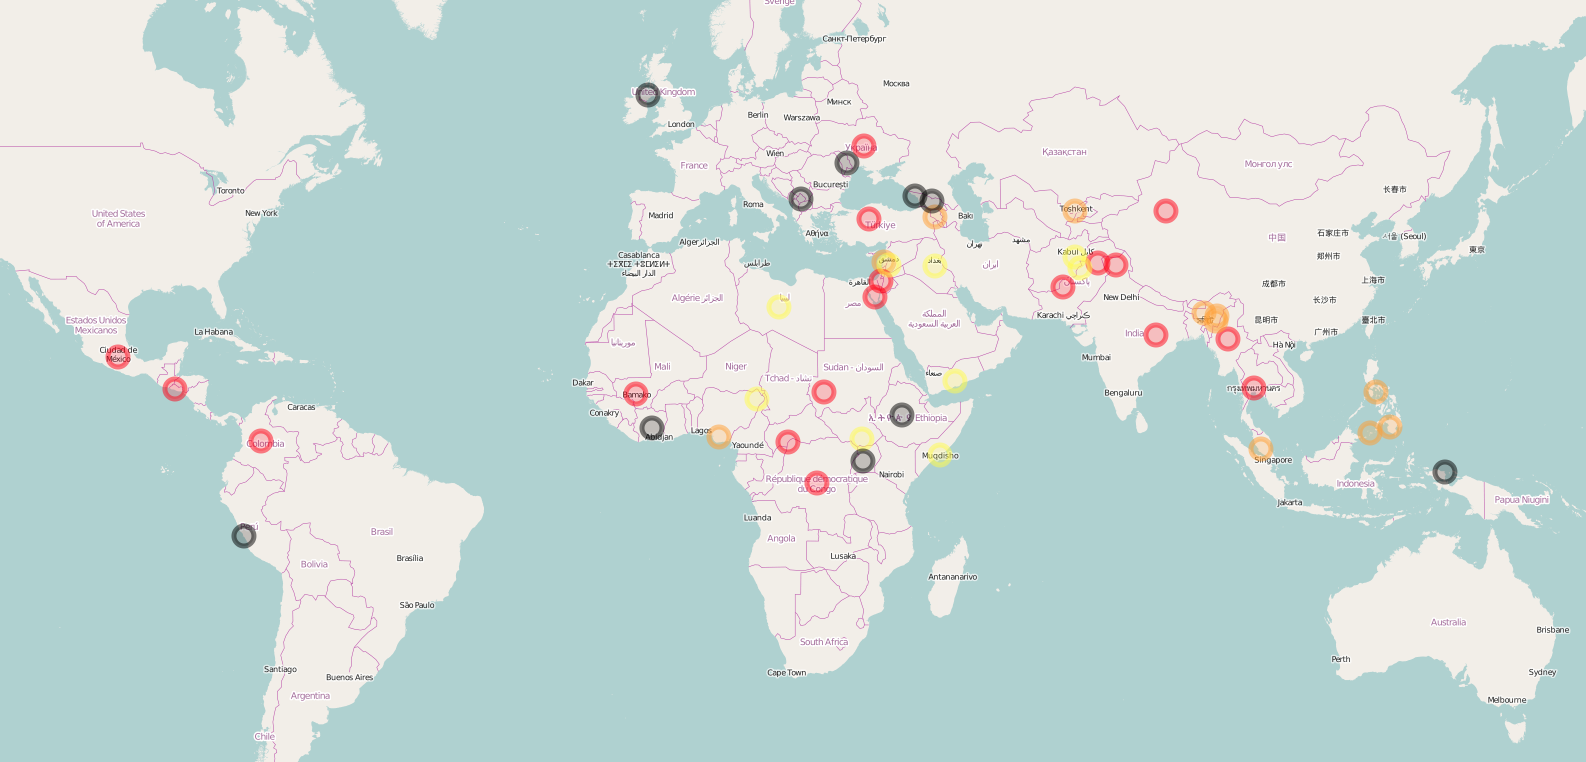
\includegraphics[width=0.9\columnwidth]{map}
\caption{A map of the 48 conflicts. Black, yellow, orange and red circles indicate the current level of intensity as rated by the Armed Conflict Database: archived, low, medium and high, respectively.}
\label{conflicts}
\end{figure}
\section{Research Questions}
Our research questions aim to discover how people in the West, specifically, perceive armed conflicts. The way people perceive armed conflicts is at least partially a reflection of Western news cycles, and the way they talk about them is a reflection of their perception. However, which features of the conflicts cause these perceptions in the first place? Are they the same features that have been linked to news reporting?

Reddit, being a large, mostly Western community with somewhat homogenous viewpoints (compared to other data sources like Twitter) gives an interesting outlet to answer such questions. Over a large dataset, we will focus on asking simple questions with clear answers and then using those answers to integrate with what's already been studied about social phenomena such as news cycles and network effects of news distribution. 

Thus, there are two main features of the comments we find interesting. The first is the \textit{sentiment}. Using the sentiment analyzer bundled with StanfordNLP\cite{stanfordnlp}, we rated over 25,000 comments as Very Negative, Negative, Neutral, Positive, or Very Positive. The second is the \textit{acceptability}. The acceptability references how the community perceives the comment, and thus that sentiment. 

From our exploratory data analysis, sentiment did not appear to be correlated with acceptability. We decided this meant that it was better to ask questions of negative sentiment and positive sentiment individually. We wanted to examine several factors that are related to what would affect reports discussing the conflict, with the thought that they might also influence how people discuss them.

\begin{enumerate}
\item{\textbf{Severity.} This includes the total number of people who were killed, made refugees, or internally displaced as a result of the conflict} 
\item {\textbf{Location.} There are six major regions that the Armed Conflict Database groups conflicts into.} 
\item {\textbf{Recent Severity.} This includes the number of people who were killed, made refugees, or internally displaced the same year the comment was made. In other words, do recent fatalities salience cause them to be treated differently than former fatalities?}
\item {\textbf{Age.} The number of years ago the conflict started.}
\item {\textbf{Nature.} What characterizes the conflict? Why did it start?}
\item {\textbf{Expert Perception.} The Armed Conflict Database rates conflicts for their current level of intensity. While this is obviously correlated with deaths, refugees, and IDP ($p < 0.0001$), the average person may be more likely to get their ideas of severity from experts, rather than numbers} 
\end{enumerate}


\section{Methods}
\subsection{Data Preparation}
We had to solve several problems in order to answer our research questions. First, how do we determine if a comment is about a specific conflict? Next, how do we determine whether that comment is positive or negative? Lastly, how do we determine whether the community found that comment acceptable or not?

To determine if a comment was about a given conflict, we compiled a list of keywords . The goal of this list was to be broad enough to capture any given comment while also ensuring that comments would be a positive identification of the topic. It is of course impossible to avoid both false positives and false negatives. It is a near guarantee that some comments tagged would not actually pertain to the given conflict. Our answer to this is to use enough data to filter out most of the noise. The biggest source of comments was /r/worldnews, with many of the others coming from similar subreddits, implying that most of the comments were likely about the intended topic. The comments came from over a thousand subreddits; some of these could be falsely identified to be relevant, while some of them could be off topic. 

As discussed earlier, we ran sentiment analysis on the comments we collected. Interestingly, there were many more negative comments than positive comments. It is possible that this is due to the subject matter; in general, pity and sadness might be more common responses to tragedy than optimism and hope. It could also be due to the nature of the corpus itself: young people on pseudononymous Internet communities are perhaps more negative than normal (NEED A CITATION HERE?). Nonetheless, we separated the negative and positive comments and pruned the neutral ones.

Lastly, we must define what it means to be acceptable. In Reddit, this is quite simply looking at whether a comment has been upvoted or downvoted more. (IS THIS SENTENCE RIGHT?) All comments start with a score of one; the idea is that you always approve of your own comment. As comments with a score of one thus contain no useful information about how the community perceived them, they were excluded. Due to Reddit hiding downvoted comments and elevating upvoted comments, we decided that the actual value of the rating is not that important. (I DO NOT FULLY UNDERSTAND WHY IT IS NOT THAT IMPORTANT.) Posts that were both upvoted and downvoted (deemed controversial by Reddit) (CAN JUST SAY CONTROVERSIAL AS YOU MENTIONED BEFORE IN THE REDDIT CORPUS) were vanishingly small, making up less than 2\% of the filtered comments. Thus, people clearly tend to downvote comments that were already downvoted and upvote comments that were already upvoted (or to take no action at all). Therefore, a binary value of approval seemed more appropriate than any other choice.

These two filters resulted in 781 positive comments and 14289 negative comments. The substantial difference in sentiment made splitting the analysis a must. Comparing these two models could help us determine if there are different circumstances when being positive is more acceptable. Due to the overwhelming number of negative comments (over 95\%), it is difficult to interpret the negative sentiment as much more than the norm. If this is the case, then our results, instead of reflecting when negative sentiment would be acceptable, would reflect when posters are more likely to post something that is unacceptable. We'll discuss what that might mean later.

\subsection{Model}
We use a Logistic Linear Mixed Effects Model (GLMM) to attempt to explain which sentiments were acceptable as determined by the conflict.

SHOULD THAT BE GENERALIZED LINEAR MIXED EFFECTS MODEL??

\subsubsection{Response}
Every comment is coded as either unacceptable (1) or acceptable (0). This means that for some feature of a conflict that a comment is about, positive $\beta$ implies that comment is more likely to be disapproved of. Conversely, negative $\beta$ implies that comment is less likely to be disapproved of. 

\subsubsection{Fixed Effects}
\begin{itemize}
\item{\textbf{Refugees.} The total number of refugees from the conflict.}
\item{\textbf{Fatalities.} The total number of fatalities from the conflict.}
\item{\textbf{IDP.} The total IDP from the conflict.}
\item{\textbf{Intensity.} The current intensity of the conflict, according to the Armed Conflict Database. The possible values are Low, Medium, High, or Archived (no current violence).}
\item{\textbf{Same Year Refugees. The number of new refugees from that conflict the year the comment was made.}}
\item{\textbf{Same Year IDP. The number of Internally Displaced Persons the year the comment was made.}}
\item{\textbf{Same Year Fatalities. The number of fatalities that occurred the year the comment was made. }}
\item{\textbf{Age.} The number of years since the violence started until today.}
\item{\textbf{Foreign Involvement.} Whether the conflict involved a foreign actor as a main antagonist. For instance, this would include the War in Iraq, but it would not include interventions by UN Peacekeepers. This was self-coded.}
\item{\textbf{Separatist Conflict.} Whether the conflict was characterized by groups wishing to secede, according to the Armed Conflict Database.}
\item{\textbf{Territorial Conflict.} Whether the conflict was characterized by two countries fighting over territory, according to the Armed Conflict Database.}
\item{\textbf{Terrorism.} Whether the conflict was characterized by terrorist activity, according to the Armed Conflict Database.}
\item{\textbf{Ethnic Conflict.} Whether the conflict was characterized by ethnic or sectarian violence, according to the Armed Conflict Database.}
\item{\textbf{Criminal Violence.} Whether the conflict was characterized by criminal activity, according to the Armed Conflict Database.}
\item{\textbf{Region.} These include the total number of fatalities that have occurred as a result of the conflict, the current Internally Displaced Persons (IDP) from the conflict, and the current number of Refugees from the conflict.}
\end{itemize} 

MAKE REGION AND AGE CONSISTENT WITH BEFORE.

\subsubsection{Random Effects}

Intercepts grouped by... (...?)
\begin{itemize}
\item{\textbf{Author.} As Reddit is pseudononymous, some authors may have a reputation for making consistently good or bad posts.}
\item{\textbf{Subreddit.} What is acceptable in one subreddit may be unacceptable in another.}
\end{itemize}

\section{Results}
\subsection{Positive}
Unfortunately, the positive comments were too few in number to get effective results. This could change upon the addition of more comments. The goal of analyzing the positive comments is to determine when it is acceptable to have positive sentiment.

IS THERE A LITTLE MORE TO SAY HERE?

\subsection{Negative}
The goal of analyzing the negative comments is to determine when it is acceptable to have negative sentiment. Obviously, negative sentiment when it comes to something like armed conflict is a fairly broad idea. Negative sentiment could potentially include anything from hateful to depressed. Nonetheless, the score unambiguously reflects the community's acceptance of that negativity.

Due to the number of variables, several models were created separately to avoid rank deficiency. Intensity (the code by the Armed Conflict Database) had a significant positive linear effect ($p < 0.05$), implying that the higher the intensity, the more likely negative comments were to be disapproved of. Age was also significant, showing a negative effect (older conflicts were less likely to be disapproved of), but the interaction among them was not.

No variables based on externalities that occurred the same year as the conflict were significant.

No variables based on current total externalities were significant.

There was a significant positive effect on Foreign involvement, implying comments were more likely to be disapproved of if there were foreign actors at play. There was also a significant positive effect if the armed conflict was largely Criminal in nature, but there was a very significant negative effect if the conflict was Separatist in nature (implying that it's unlikely that comments expressing negative sentiment were disapproved of).

For region, there was a very significant negative effect on both Europe and East Asia.
\section{Discussion}
There are several ways to interpret the rate of unacceptable posts for any given conflict. As the majority of Reddit users are fairly homogeneous in opinion, it is possible that people vary how likely they are to make posts about certain topics when they know that many people will disapprove. This could stem from \textit{passion} about a topic: someone feels it is more important to speak their mind than to have a popular post. Alternatively, it could reflect \textit{dissent}; while there might not be enough dissenters to affect the gatekeeping system, the willingness to express something others disapprove of at all suggests there are some who disagree with the majority opinion. 

\subsection{Negative Sentiment}
Due to the vast majority of comments being of negative sentiment, we assume it is the default way to respond to a conflict. Thus, we will consider the Negative Sentiment model the same as the Default model.

The Regions of East Asia/Australasia and Europe both have reliable negative predictors. This implies the rate of disapproval when discussing these topics is very low. This is somewhat unsurprising given the general demographics of Reddit. Users from those regions, due to comparable socioeconomic status or military alliances, may see themselves as similar, prompting a homophily effect. The lack of significant effects for the other regions could be because commenters conflate areas with which they are less likely to empathize, such as the Middle East/North Africa and SubSaharan Africa.

The negative effect of Age makes sense from the perspective of passion. While many people may have an opinion on older conflicts, these feelings may be less immediate due to the numbness or weariness of prolonged violence.

Territorial disputes on the other hand, are logically controversial. To those whose country plays a role or are immediately affected by them, they may seem very important. However, to those farther away, they could seem like petty bickering.

Interestingly, the objective variables, such as Fatalities and IDP, played almost no role in the model. Absence of evidence is not evidence of absence; however, this integrates well with previous work \cite{Berinsky2009}.

\subsection{Positive Sentiment}
We can assume positive sentiment corresponds to hope, optimism, or perhaps even sarcastically phrased misanthropic sentiments. For instance, in the case of comments about conflicts with higher Fatalities being more likely to be disapproved of, it might be the latter. 

On the other hand, positive sentiment surrounding conflicts containing notes of Terrorism or Separatism may correspond to hope. For instance, they could be expressions of hope for those attempting to separate from a regime where they do not feel represented, or wishes for those who are suffering terrorism to remain steadfast. These should both be uncontroversial ideas, so it is unsurprising they are more likely to be considered acceptable.
%One possible interpretation of unacceptable posts Reddit users to post in anger. If Reddit is fairly homogenous in viewpoint, as a lack of controversial comments would suggest, positive correlations could reflect someone who posted something they knew would be disagreed with. In this way, someone who found the Reddit explanation of events frustrating could become angry and post a message that is likely to be downvoted. In this way, it would be sensible for Age to be negatively correlated, as fewer people are as passionate about historical events as they are about present day events.

\subsection{Future Work}
Some of the interpretation is ultimately speculative. A more fine-grained model of sentiment could potentially help us determine with more authority what is the true cause of these effects. We would further like to tie these ideas into more general cognitive and perceptual biases. For instance, one possibility of the low effect of negative externalities could be due to poor estimates of those values.
\section{Conclusion}
This paper sought to add to a growing body of work about media perception of armed conflicts by systematically investigating a large sample of Reddit data and cross-referencing the Armed Conflict Database. The vast majority of discussions are negative in tone, which is logical given the somber nature of violence. Among these, comments were less likely to be disapproved of if they were from the same demographic as the majority; they were more likely to be disapproved of if they concerned a Territorial Dispute or were older. We consider this study as preliminary evidence of the effect of perceptual biases in viewing conflicts. These biases are important due to the public's role in shaping foreign policy.
\section{Acknowledgements}
This research was supported by a grant from the National Science Foundation (SBE-SES-1528624) to D.R. titled ``Updating the Militarized Dispute Data Through Crowdsourcing''.

\bibliographystyle{splncs03}
\bibliography{review,nlp,reddit}


\end{document}
